\documentclass[tikz,border=6pt]{standalone}
\usepackage{tikz}
\usetikzlibrary{arrows.meta}
\usepackage[T1]{fontenc}

\definecolor{primary}{HTML}{6B4FA0}
\definecolor{highlight}{HTML}{C4664A}
\definecolor{muted}{HTML}{8A7A9B}

\tikzset{
  % Thicker outlines and larger inner sep than the full logo — legible at small sizes
  gate/.style={circle, draw=#1, fill=#1!15, line width=1.2pt,
    inner sep=5pt, font=\large\bfseries, text=#1},
  wire/.style={line width=1.0pt, muted!90, -{Stealth[length=3.5pt,width=3pt]}}
}

\begin{document}
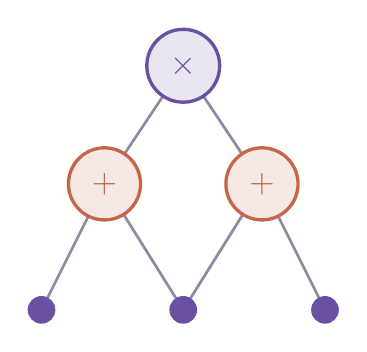
\begin{tikzpicture}

\def\baseY{0}
\pgfmathsetmacro{\pY}{\baseY+1.6}
\pgfmathsetmacro{\xY}{\baseY+3.1}

% Wires (drawn first)
\draw[wire] (-1.8,\baseY) -- (-1.0,\pY);
\draw[wire] (   0,\baseY) -- (-1.0,\pY);
\draw[wire] (   0,\baseY) -- ( 1.0,\pY);
\draw[wire] ( 1.8,\baseY) -- ( 1.0,\pY);
\draw[wire] (-1.0,\pY)    -- (0,\xY);
\draw[wire] ( 1.0,\pY)    -- (0,\xY);

% Dots (on top of wires)
\foreach \x in {-1.8, 0, 1.8} {
  \fill[primary] (\x,\baseY) circle (5pt);
}

% Gates (on top of wires)
\node[gate=highlight] at (-1.0,\pY) {$+$};
\node[gate=highlight] at ( 1.0,\pY) {$+$};
\node[gate=primary]   at (   0,\xY) {$\times$};

\end{tikzpicture}
\end{document}
